%%%%%%%%%%%%%%%%%%%%%%%%%%%%%%%%%%%%%%%%%
% Medium Length Professional CV
% LaTeX Template
% Version 2.0 (8/5/13)
%
% This template has been downloaded from :
%  http://www.LaTeXTemplates.com
%
% Original author :
% Trey Hunner ( http://www.treyhunner.com/)
%
% Important note :
% This template requires the resume.cls file to be in the same directory as the
% .tex file. The resume.cls file provides the resume style used for structuring the
% document.
%
%%%%%%%%%%%%%%%%%%%%%%%%%%%%%%%%%%%%%%%%%

%----------------------------------------------------------------------------------------
%	PACKAGES AND OTHER DOCUMENT CONFIGURATIONS
%----------------------------------------------------------------------------------------


\documentclass{resume} % Use the custom resume.cls style
\usepackage[utf8]{inputenc}
\usepackage[left=0.75in,top=0.6in,right=0.75in,bottom=0.6in]{geometry} % Document margins
\usepackage{hyperref}
\usepackage{footnote}
\usepackage{pifont}
\usepackage{graphicx}

\usepackage{xcolor}
\usepackage[normalem]{ulem} 			% \sout macro
\usepackage{amssymb}

\newboolean{showcomments}
% \setboolean{showcomments}{false}
\setboolean{showcomments}{true}


% ********************************************************************* 
% Revisions and comments Macros
% ********************************************************************* 
	
\ifthenelse{\boolean{showcomments}}
{
	\newcommand{\nb}[3]{
		{\colorbox{#2}{\bfseries\sffamily\scriptsize\textcolor{white}{#1}}}
		{\textcolor{#2}{\textsf\small$\blacktriangleright$\textit{#3}$\blacktriangleleft$}}}
	 \newcommand{\version}{\emph{\scriptsize$-$Id$-$}}
	\newcommand{\bnote}[2]{\fbox{\color{blue}\bfseries\sffamily\scriptsize#1}
    	{\color{blue}\textsf\small$\blacktriangleright$\textit{#2}$\blacktriangleleft$}}
	\newcommand{\old}[1]{{\color{gray}\sout{#1}}} % old to be removed
	\newcommand{\del}[1]{\old{#1}} % please remove
	\newcommand{\ins}[1]{{\textcolor{blue}{\uline{#1}}}} % please insert	
	\newcommand{\ugh}[1]{{\textcolor{red}{\uwave{#1}}}} % please rephrase	
	\newcommand{\chg}[2]{{\textcolor{red}{\sout{#1}}}{\ra}\textcolor{blue}{\uline{#2}}} % please change
	\newcommand{\here}{\bnote{***}{CONTINUE HERE}} 
	\newcommand{\fix}[1]{\bnote{FIX}{#1}}
}{
	\newcommand{\bnote}[2]{}
	\newcommand{\nb}[3]{}
	\newcommand{\old}[1]{}
	\newcommand{\del}[1]{}
	\newcommand{\ins}[1]{}
	\newcommand{\ugh}[1]{}
	\newcommand{\chg}[2]{}
	\newcommand{\here}{}
	\newcommand{\fix}[1]{}
} 

\newcommand{\hide}[1]{}

%---% add your own macros 
\newcommand{\luc}[1]{\nb{Luc}{blue}{#1}}
\newcommand{\noury}[1]{\nb{Noury}{red}{#1}}
\newcommand{\sd}[1]{\nb{Stef}{orange}{#1}}
\newcommand{\pablo}[1]{\nb{Pablo}{orange}{#1}}
\newcommand{\gp}[1]{\nb{Guille}{orange}{#1}}
\newcommand{\santi}[1]{\nb{Santi}{orange}{#1}}
%---







\name{Fiches de mission} % Your name

	\address{28 rue Clovis Hugues \\ Lille, 59800 } % Your address
	\address{(+33)~$\cdot$~7~$\cdot$~83~$\cdot$~14~$\cdot$~45~$\cdot$~35 \\ santiagobragagnolo@gmail.com} % Your phone number and
	\address{Santiago Bragagnolo } % Your address
\begin{document}


\section{Donn\'{e}es Biographiques}

\begin{itemize}
	\item Pr\'enom et Nom: Santiago Pablo Bragagnolo  
	\item Date de naissance: 16 novembre 1982  
	\item Nationalités: Argentine, Italienne  
\end{itemize}



\section{Contact}

\begin{itemize}
	\item Skype: santiago.bragagnolo  
	\item Linkedin: linkedin.com/in/santiagobragagnolo/  
	\item Portfolio: santiagobragagnolo.wordpress.com  
	\item Blog: knowledgeconvergence.wordpress.com  
	\item Github: github.com/sbragagnolo 
\end{itemize}


%----------------------------------------------------------------------------------------
%	MISSION AUFIERO
%----------------------------------------------------------------------------------------


\section{Fiche de Mission I - Aufiero Informatica S.R.L.}



	La premi\`ere mission que j'ai choisi de pr\'esenter est ma mission industrielle la plus repr\'esentative, durant la période mars 2007 - décembre 2010. C'est l'entreprise qui m'a form\'e le plus sur le développement logiciel industriel. J'ai fait évoluer mes aptitudes techniques aussi que humaines. 
	Aufiero Informatica S.R.L. est une entreprise moderne de taille petite-moyenne (dix \`a quinze personnes), avec une organisation matricielle ou par project : sans beaucoup de hiérarchies, mais avec beaucoup des projets. 


 \begin{figure}[!htp]
 \begin{center}
 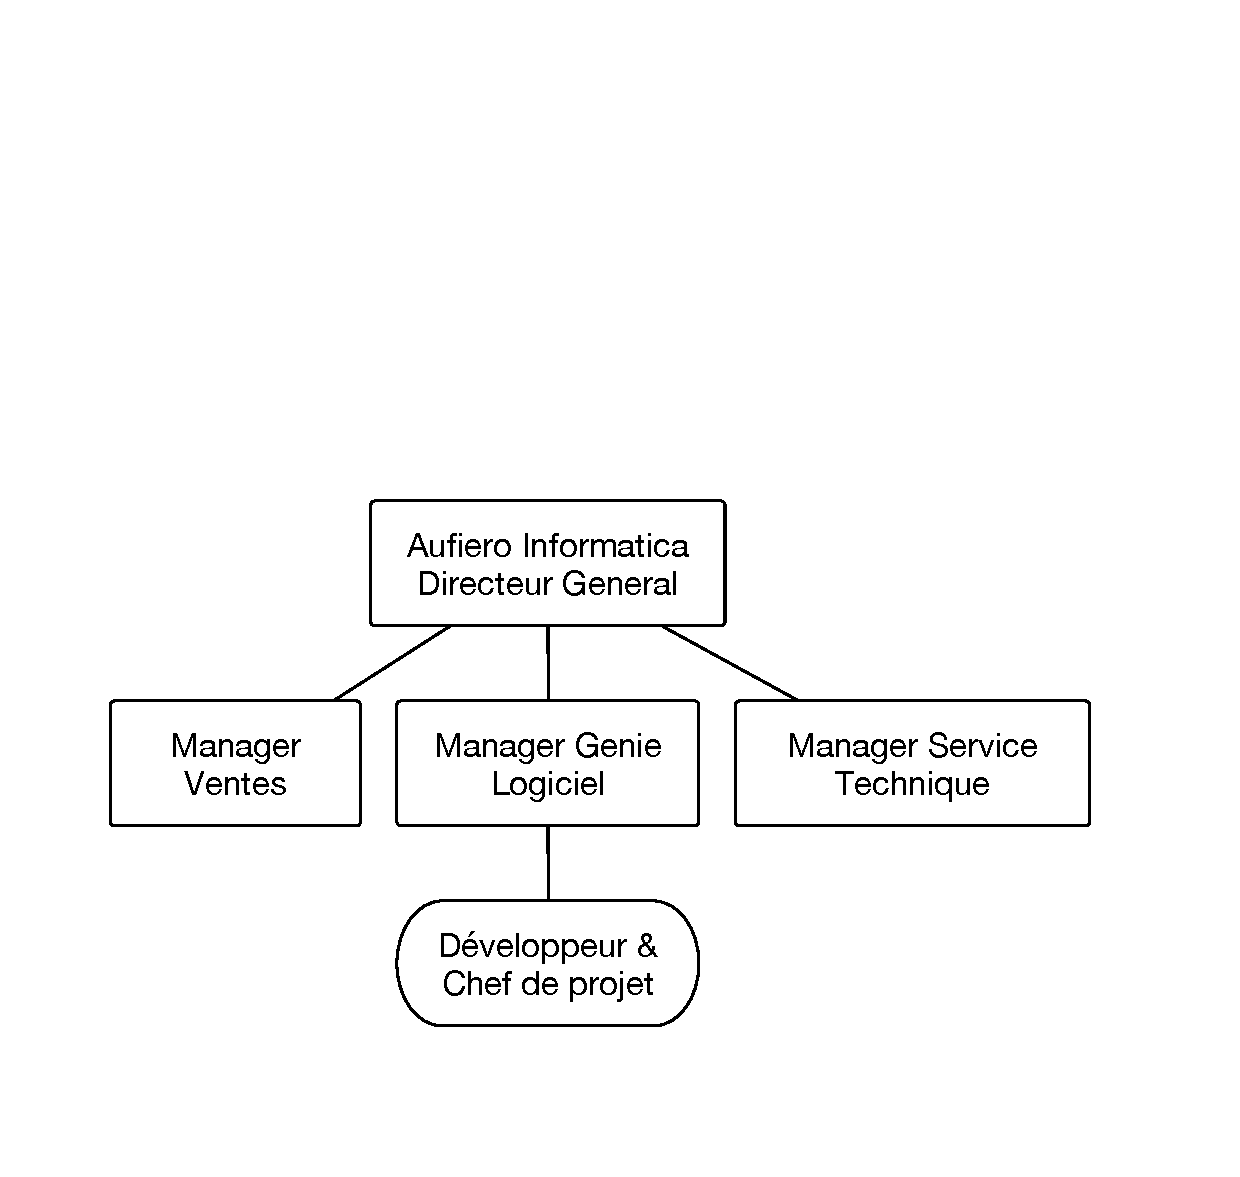
\includegraphics[width=0.60\linewidth]{aufiero.pdf}
 \caption{Aufiero}
 \end{center}
 \end{figure}
		
	\subsection{Responsabilités}

\newcommand{\uno}{\ding{172}\ }
\newcommand{\dos}{\ding{173}\ }
\newcommand{\tres}{\ding{174}\ }
\newcommand{\cuatro}{\ding{175}\ }

\newcommand{\UNO}{\ding{202}\ }
\newcommand{\DOS}{\ding{203}\ }
\newcommand{\TRES}{\ding{204}\ }
\newcommand{\CUATRO}{\ding{205}\ }


\begin{table}[!htbp]
\label{table-aufiero}
\begin{tabular}{|l|l|l|l|l}
\cline{1-4}
   & Descriptif des tâches &  \% & Niveau de Responsabilité \footnotemark &  \\ \cline{1-4}
 A& Interaction avec un client permanent & 20\% & 4 &  \\ \cline{1-4}
 B& Conception / Développement sur systèmes d'un client permanent & 30\%& 4&  \\ \cline{1-4}
 C& Administrateur de base de données  & 10\%  & 3 &  \\ \cline{1-4}
 D& Architecte et planning d'applications sur de nouveaux projets & 25\% & 3 &  \\ \cline{1-4}
 E& Conception / Développement sur de nouveaux projets & 15\% &2&  \\ \cline{1-4}
\end{tabular}

\caption{Responsabilités}
\end{table}
Dans la table \ref{table-aufiero} on peut observer mes responsabilités  \`a la fin de mon cycle dans l'entreprise.
L'ordre d'importance de mes tâches est : A - D - B - C - E. 

\footnotetext{
Niveau de responsabilité
\begin{enumerate} 
	\item de l'application de consignes ou de procédures
	\item de l'amélioration ou de l'optimisation de solutions ou de propositions
	\item de la conception de programmes ou de la définition de cahiers des charges 
	\item de la définition d'orientations ou de stratégies
\end{enumerate}
}

\subsection{Relations humaines} 

Dans cette position, j'étais fait partie de deux équipes de travail. Une équipe en charge de répondre aux  requêtes d'Oceano Argentina,  notre client le plus important. 
L'autre équipe en charge de recevoir, analyser et implémenter les nouveaux projets arrivant. 

Chacune de ces équipes m'a exposé aux différentes relations humaines et différentes relations hiérarchiques.  
Oceano Argentina est une des succursales du Grupo Oceano, un groupe éditorial espagnol, avec plus de 50 ans de trajectoire. 
Avec un taille moyenne en argentine d'autour de 100 personnes, les responsabilités principales d'Oceano Argentina sont la vente, marketing et distribution de livres en Argentine et en Uruguay. 


 \begin{figure}[!htp]
 \begin{center}
 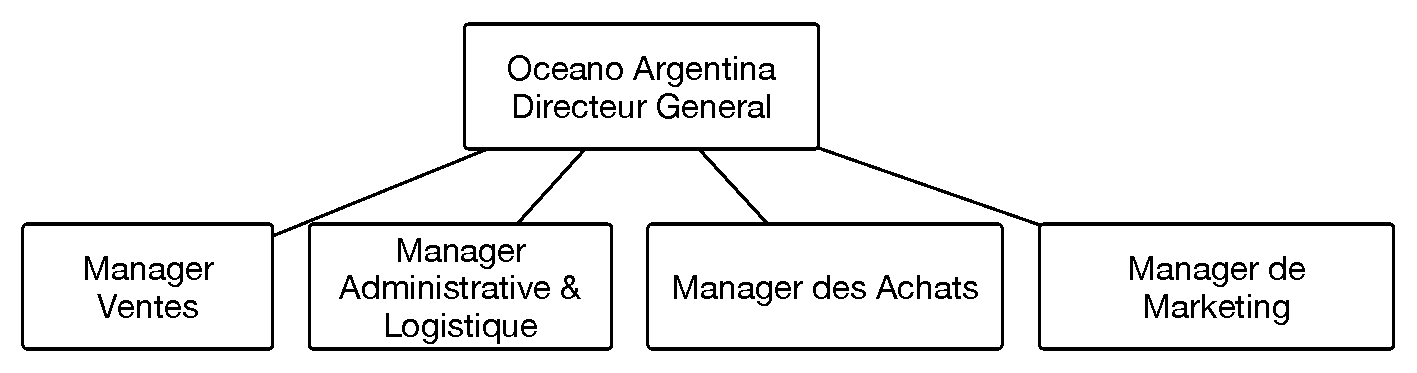
\includegraphics[width=0.60\linewidth]{oceano.pdf}
 \caption{Oceano}
 \end{center}
 \end{figure}

	
	\subsubsection{Relations hiérarchiques} 
	

		\paragraph{Dans l'équipe d'Oceano Argentina,} j'ai été chef de projet logiciel, et des services d'infrastructure.  Notre équipe a été en charge de la maintenance des systèmes pre-existants, réseaux, base de données et infrastructure hardware. 
		
		\begin{enumerate}
		\item \textbf{De qui recevez-vous vos objectifs, vos instructions?}
			Les objectifs de cette équipe ont été définis dans les reunions annuelles et mensuelles entre le directeur d'Aufiero Informatica S.R.L, le manager de logistique, le manager de ventes, et moi.
		\item \textbf{Sous quelle(s) forme(s)?}
			Le résultat de chaque réunion mensuel a été un cahier des charges numérique, avec les tâches par mois, leurs estimations et les priorités. Ce cahier de charges numérique  a été en forme de tableau.
		\item \textbf{Qui évalue votre travail?}
			Les personnes en charge d'évaluer mon travail ont été  le manager de logistique, le manager de ventes et le directeur d'Aufiero Informatica S.R.L. 
		\item  \textbf{Éventuellement à qui donnez-vous des objectifs. des instructions, des consignes ?}
			J'ai donné des objectifs au service de maintenance de réseaux et infrastructure hardware (rénovation et réparation des ordinateurs, serveurs, imprimantes, etc).
		\item \textbf{Sous quelle(s) forme(s)?}
			Sous le format d'ordres de travail électroniques fourni pour Aufiero Informatica S.R.L, et aussi en format courriel. L'estimation de chaque tâche a été responsabilité du personnel d'infrastructure. 
			J'\'etablissais les priorités en collaboration avec le manager responsable et le directeur d'Aufiero Informatica S.R.L.  
		\item \textbf{Comment évaluez-vous l'activité de vos collaborateurs}
			Pour évaluer l'activité de mes collaborateurs, j'ai utilisé principalement des réunions informelles hebdomadaires et le retour du personnel d'Oceano Argentina. 
		\end{enumerate}
		
		\paragraph{Dans l'équipe de nouveaux projets,} j'ai été architecte logiciel. Mon rôle principal a été la  prise de décisions d'architecture et conception général des nouvelles solutions informatiques, suivre leur développement et garantir leur qualité. 
		
		\begin{enumerate}
		\item \textbf{De qui recevez-vous vos objectifs, vos instructions?}
			Mes objectifs ont été définis en collaboration pour le chef de projet et les clients.
		\item \textbf{Sous quelle(s) forme(s)?}
			Forme orale, pendant les réunions de planification, et suivi dans un logiciel de planification de projets.
		\item \textbf{Qui évalue votre travail?}
			J'ai été évalué périodiquement dans les réunions de sprint et de fin de projet, pour tout l'équipe, mais principalement par le chef de projet. 
		\item  \textbf{Éventuellement à qui donnez-vous des objectifs. des instructions, des consignes?}
			Dans cette équipe je n'avais pas de  personnes \`a charge, mais \textbf{j'ai été le référent technique}.
		\end{enumerate}
		
					
	\subsubsection{Relations horizontales}
	
	
		\paragraph{Dans l'équipe d'Oceano Argentina,}
		
		\begin{enumerate}
		\item \textbf{Avec quel(s) service(s) internes êtes-vous en relation pour l'exécution de cette mission?}
			Dans l'équipe d'Oceano Argentina, mon travail a été articulé  avec  les différents départements de l'entreprise client. 
			J'ai travaillé en relation horizontale spécialement avec le manager de logistique et d'achats, le manager de ventes, et en moindre proportion, avec le manager de marketing. 

		\item \textbf{Sous quelle(s) forme(s)?}
			Le but général de notre collaboration a été la définition des objectifs et la mise en place des mises \`a jour et nouvelles fonctionnalités. 
		Les moyens d'organisation ont été principalement des réunions et des échanges par courriels. 
		\end {enumerate}	
		
		\paragraph{Dans l'équipe de nouveaux projets arrivent,} mon travail a été plusieurs fois lié aux départements de ventes et marketing. 
		
		\begin{enumerate}
		\item \textbf{Avec quel(s) service(s) internes êtes-vous en relation pour l'exécution de cette mission?}
			Chef de ventes et marketing. 
		\item \textbf{Sous quelle(s) forme(s) ?}
			Couramment de façon orale ou courriel et pendant des réunions ou de journées de travail en équipe.
		\end{enumerate}

	
	\subsubsection{Relations extérieures} 
		\paragraph{Dans l'équipe d'Oceano Argentina,} nous avions des relations avec les fournisseurs de stockage de livres (Les dépôts de livres ont été externalisés).
		\begin{enumerate}
		\item \textbf{Avec quel(s) partenaire (s) êtes-vous en relation pour l'exécution de cette mission?}
			J'ai été en contact avec le manager de compte d'Oceano Argentina, avec qui on faisait la consolidation des stocks une fois par an.
		\item \textbf{Sous quelle(s) forme(s)?}
			Téléphone et courriel ont été les moyen principaux de communication. 
		\item \textbf{Avec quelle fréquence?}
			Au besoin, spécialement pendant la fin de l'année commercial.
		\end {enumerate}			
		
		\paragraph{Dans l'équipe de nouveaux projets,} j'avais des relations avec les clients, nécessaires pour arriver \`a comprendre les fonctionnalités demandées.   
		\begin{enumerate}
		\item \textbf{Avec quel(s) partenaire(s) êtes-vous en relation pour l'exécution de cette mission?}
			Les clients.
		\item \textbf{ Sous quelle(s) forme(s)?}
			Téléphone et courriel et pendant les réunions d'avancement 
		\item \textbf{Avec quelle fréquence?}
			Une fois par mois.
		\end {enumerate}			
		
	\subsection{Décrivez les principales qualités que vous avez eu \`a mobiliser dans cette mission}
	
		\begin{itemize} 				
			\item \textbf{Autonomie} \newline
				J'ai eu la responsabilité de d\'efinir mes propres priorités, comme résultat de rester beaucoup de temps chez notre principal client, et être la seule personne qui comprend les besoins de l'entreprise et au même temps les co\^uts techniques de chaque tâche.
			\item \textbf{Créativité et Pragmatisme } \newline
				Etre dans les réunions de définition des tâches m'a exposé au management des budgets et temps de projet. Au niveau du management, cela m'a aidé \`a  dimensionner les problèmes, et comprendre le type de solution dont nous avions  besoin. Par défaut on veut toujours la meilleure solution. Mais, en regardant le budget, il faut bien choisir et comprendre quel est le bon compromis, et comment faire pour résoudre  les problèmes de la mani\`ere la plus simple et \'efficace. 
			\item \textbf{Curiosité } \newline
				La curiosité est probablement une des qualités plus importantes d'un bon architecte d'applications. Connaitre les différents outils et solutions du marché, et comprendre comment les utiliser pour résoudre les différents problématiques.
			\item \textbf{Autodiscipline} \newline
			Pouvoir être curieux, et en même temps suivre le chemin du pragmatisme, et pouvoir suivre le plan dessin\'e pour moi-même, m'a demandé être  beaucoup d'autodiscipline.
			\item \textbf{Négociation  et prise de décision } \newline
				Étant la personne qui définit mes propres tâches avec des grosses figures du client, m'a poussé \`a adopter une position de négociation avec une fréquence mensuelle, et plusieurs fois pour mois dans une situation de prise de décision.  
		\end{itemize}
		
	\subsection{Pouvez-vous présenter une situation-problème que vous avez eu a résoudre dans le cadre de cette mission et la façon de dont vous avez procédé?}
	
		Sans doute les problèmes plus sérieux que me sont arrivés sont du coté d'Oceano Argentina. 
		Annuellement, \`a Buenos Aires a lieu un événement très important, spécialement pour des entreprises comme Oceano Argentina. Cet événement est "la Feria del Libro" (la foire du livre). 
		Dans cet événement on installe chaque année un "stand" de vente et diffusion, pendant la durée d'un mois. 	
		Le développement de ce poste de ventes est probablement le problème le plus hétérogène et aussi le plus intéressant. 
		
		\paragraph{ Sur le contexte } 
		
		Oceano Argentina est un \'editeur. 
		
		\begin {itemize} 
		 \item Leur clients conventionnels sont des librairies de toutes tailles.
		 \item Chaque client a un compte de système.
		 \item Oceano Argentina ne vend pas des livres au consommateur final.
		\end{itemize}
		
		Le système a été développé pour un process très spécifique 
		\begin{itemize} 
		   \item Le système de gestion a été conçu pour un processus de vente qui divise la vente faite par les vendeurs de l'enregistrement de la vente.
		   \item Le système de gestion avait plusieurs types d'utilisateurs avec des roles bien différents.
		   \item Le système de gestion ne permet qu'une seule session ouverte \`a la fois.
		   \item Le système de gestion a été  sensé \`a imprimer des donn\'ees sur des factures vides, avec un format spécifique, avec une technologie d'impression non standard.
		   \item Le système de gestion a été déployé sur un réseaux privé, isolé des acces internet.
		   \item Le système de gestion travaille sur une base de données centralisée.
		\end{itemize} 
		
		Cette nouvelle configuration lors de la fête du livre pr\'esente un grande nombre des problémes fonctionnels, opérationnels et d'infrastructure  qui n'existe pas le reste de l'année. C'est a dire: 
		
		\paragraph{Infrastructure}
		\begin {itemize} 
			\item Le bâtiment o\`u se déroule l'événement n'offrait aucun service d'access \`a internet suffisamment stable, sécurisé et fiable
		\end {itemize}
		\paragraph{Fonctionnelle}
		\begin {itemize} 
			\item Pour des impositions légales, il fallait utiliser une imprimante fiscale.
			\item Le système devait marcher avec plusieurs vendeurs au même temps.
			\item La interface graphique devait présenter une interaction fluide pour des livres individuelles 
		\end {itemize}
		\paragraph{Opérationnelles}
		\begin {itemize} 
			\item Le poste devait être indépendant 
			\item Les mouvements fiscals et de stock du système devaient être visibles pour tous les utilisateurs.
		\end {itemize}		
		
		
		
	   \paragraph{La solution apportée} pour le problème a demandé beaucoup d'efforts et la mise en place d'une serie de  processus  pour mettre en place le point de vente au stand.
	   
	       Cette solution avait deux axes principaux que je vais présenter et développer ci-dessous
	   
	  	        
		\paragraph{Axe I: Infrastructure}
			Le système de gestion imposait l'utilisation d'une base de données centralisée comme restriction, et que cette base de données ne pouvait pas être consultée de manière fiable via l'infrastructure réseau fournie par le site.
La solution la plus efficace et la moins coûteuse a été  l'installation et la mise en place d'un réseau dédié nécessaire pour répondre aux besoins d'installation du système de gestion.

Cette solution amène avec elle le problème de la synchronisation de la base de données du poste avec la base de données utilisée par le système général de l'entreprise. Ce problème est partiellement résolu dans l'axe de développement logiciel.

Enfin, pour améliorer la réponse du système de gestion et protéger les informations confidentielles de nos clients, nous avons décidé d'utiliser une version réduite de la base de données productive, qui contient uniquement les données nécessaires pour les ventes du stand, sans tenir compte des données clients, ventes, factures, chiffres d'affaires, etc.
	
		\paragraph{Axe II: Développement logiciel}	
Étant donné que les bons de commande, les factures et les mouvements de stock devaient être enregistrés  afin de respecter les processus de vente, j'ai développé un module de vente qui générait et traitait la commande, la facturation et livraison de produits en même temps.
Le module inclus également la fonctionnalité d'impression des factures dans les imprimantes fiscales et le lecteur de codes-barres avec une détection ISBN de 10 et 13 caractères.
Enfin, pour résoudre le problème de la synchronisation des factures, des ventes et des mouvements de stock, j'ai développé un module d'exportation et d'importation des ventes.
La liste suivante détaille les tâches effectuées au cours du développement nécessaire.

	\subsection {Connaissances mobilisées dans cette mission }
			
	\begin{itemize} 				
			\item Technologiques 
					\begin{itemize}
						\item Architecture et conception de logiciel 
						\item Maintenance de logiciel existente
						\item Plusieurs langages de programmation (java, javascript, action script, flex, visual basic, C\# .Net, groovy, dolphin smalltalk, php, sql, t-sql)
						\item Administration de serveurs d'application (JBoss, Tomcat, Apache)
						\item Administration de bases de données (SQL Server, PL-SQL, MySql)
						\item Création et gestion de rapports et leur impression sur différentes formats et technologies hardware. (Jasper reports, cristal reports)
						\item Administration basic des serveurs de réseaux (windows et linux)
					\end {itemize}
			\item Processus \& Methodologies 
					\begin{itemize}
						\item Processus de ventes en gros et au particuliers 
						\item Processus de gestion de stocks 
						\item Methodologies agiles (planification) 
						\item Test driven development et Domain driven development
					\end {itemize}
			\item  Humains \& Sociaux  
				\begin{itemize}
						\item L'interview (avec des utilisateurs experts)
						\item Relation avec des clients
					\end {itemize}

		\end{itemize}
		


%----------------------------------------------------------------------------------------
%	MISSION ECOLE DES MINES
%----------------------------------------------------------------------------------------


\section{Fiche de Mission II - Ericsson }

 \begin{figure}[!htp]
 \begin{center}
 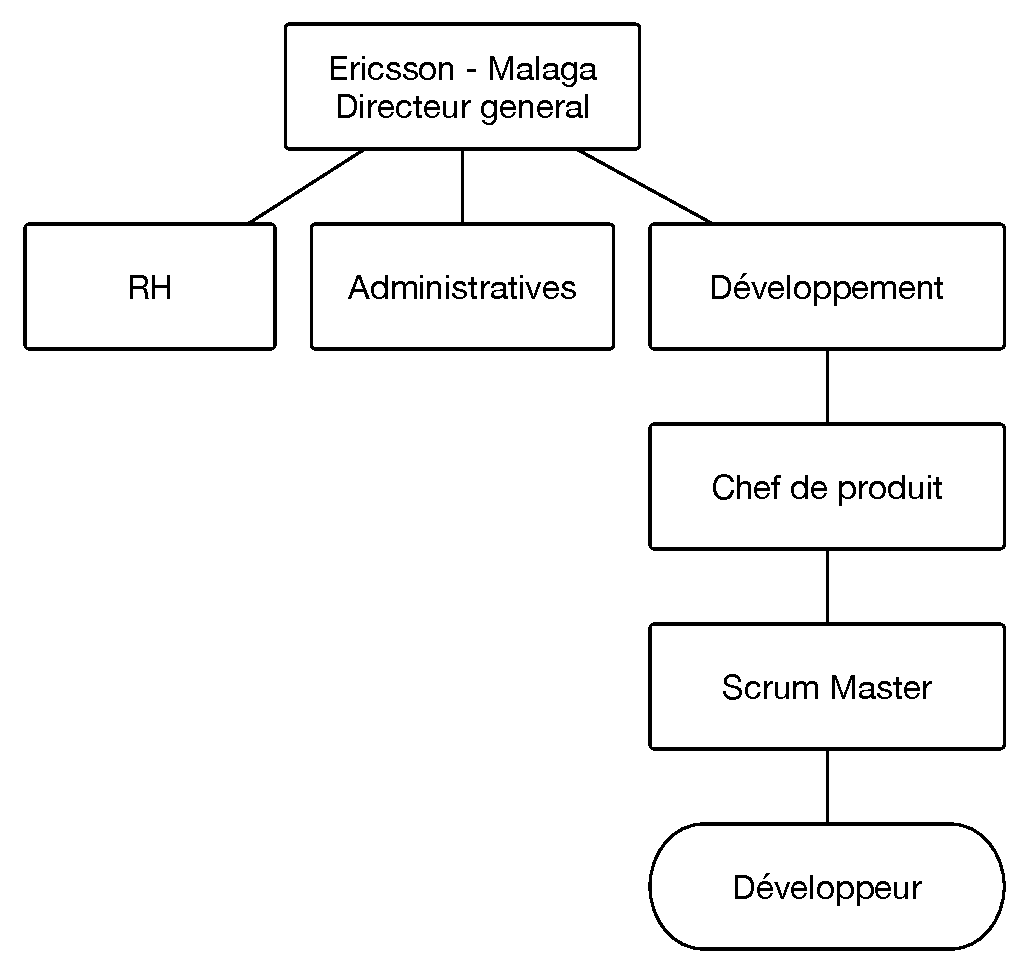
\includegraphics[width=0.50\linewidth]{ericsson.pdf}
 \caption{Ericsson}
 \end{center}
 \end{figure}

Comme deuxième mission, j'ai choisi mon expérience chez Ericsson.
Mon temps chez Ericsson n'a pas été particulièrement long, 5 mois. Le fait d'être une entreprise tr\`es reconnue,  l'emplacement du travail est dans un pays qu'est ni l'Argentine ni la France et enfin,  le domaine d'application (réseaux téléphoniques), et l'hétérogénéité des équipes, font cette mission, une mission complètement différente de mes autres expériences industrielles.

Ericsson Malaga est une filiale d'Ericsson dédiée au développement de systèmes de diagnostic de réseaux radio téléphoniques.
J'ai participé principalement dans les projets Ericsson RAN \footnotemark Analizer  (ERA), Process Trace Server (TPS), OSS Data Gateway (ODG), entre autres. 

\footnotetext{
Radio Access Network (Réseau d'Accès Radio).
}

Mon travail chez Ericsson était celui de développeur logiciel senior, travaillant dans une équipe internationale et interdisciplinaire de dix personnes, composée de:

Un chef d'équipe, deux experts en réseaux d'accès radio (RAN), cinq développeurs et trois autres personnes en qualité (QA).
Une équipe a été divisée en deux grandes parties, de première, développement, composée entièrement de développeurs et de seconde, qualité, composée d'experts RAN et QA. Chacune de ces parties a son manager.
La principale méthode d'organisation du travail était Scrum (Scrum-JIRA) avec des sprints cross-\'equipe mensuels et sprints hebdomadaires par équipe. 


\subsection{Responsabilités}
	
	
\begin{table}[!htbp]
\label{my-label}
\begin{tabular}{|l|l|l|l|l}
\cline{1-4}
   & Descriptif des tâches &  \% & Niveau de Responsabilité \footnotemark  &  \\ \cline{1-4}  
A & Conception et développement de nouvelles fonctionnalités & 40\% &3 & \\ \cline {1-4}
B & Reproduction et résolution des bugs & 30\% & 3  & \\ \cline {1-4}
C & Mise en œuvre des tests unitaires & 30\% &2   & \\ \cline {1-4}
\end{tabular}
\caption{Responsabilités}
\end{table}

L'ordre d'importance des tâches est A, B et C.


\footnotetext{
Niveau de responsabilité
\begin{enumerate} 
	\item de l'application de consignes ou de procédures
	\item de l'amélioration ou de l'optimisation de solutions ou de propositions
	\item de la conception de programmes ou de la définition de cahiers des charges 
	\item de la définition d'orientations ou de stratégies
\end{enumerate}
}
\subsection{Relations humaines}
	
	
	Pendant mon séjour à Ericsson je n'ai pas eu d'employés a ma charge, et bien que les relations hiérarchiques ait \'et\'e assez complexes, le travail de développement quotidien était plus rapide et plus organique que hiérarchique.

	\subsubsection {Relations hiérarchiques}
		\begin{enumerate}
		\item \textbf{De qui recevez-vous vos objectifs, vos instructions ?}
			Le scrum master de mon équipe, hebdomadairement, \`a travers la methodologie Scrum (Scrum-Jira)
		\item \textbf{Sous quelle (s) forme (s) ?}
			A travers le système de planification (JIRA) 
		\item \textbf{Qui évalue votre travail ?}
			Le responsable de développement de mon équipe et le scrum master de mon équipe.
		\item  \textbf{Eventuellement à qui donnez-vous des objectifs. des instructions, des consignes ?}
			Je n'ai pas eu de personnes a charge.
		\end{enumerate}


	\subsubsection {Relations horizontales}	
	\begin{enumerate}
		\item \textbf{ Avec quel (s) service (s) internes êtes-vous en relation pour l'exécution de cette mission ?}
			Les autres équipes de développement qui utilisent les m\^emes d\'ependences logicielles que nous. 
		\item \textbf{Sous quelle (s) forme (s) ?}
			Normalement sous la forme de pair programming ou de reunion informelle.
	\end {enumerate}	

	\subsubsection {Relations extérieures}
		Je n'ai pas eu de relation avec des parties extérieures dans cette mission.
		
			
\subsection{Décrivez les principales qualités que vous avez a mobiliser dans cette mission}
	
		\begin{itemize} 				
			\item \textbf{Travaille en équipe} \newline
				La taille de projet et le fait d'avoir des équipes multidisciplinaires ont permis une amélioration très importante dans ma capacité de travail en équipe. 
			\item \textbf{Methodologie} \newline
				Ericsson est de toutes les entreprises ou j'ai travaill\'e, la plus forte en application de méthodologie. Nous avons réussi \`a suivre un process Scrum bien défini pendant tout le temps que j'ai passé pour cette entreprise.  
			\item \textbf{Responsabilités  } \newline
				La définition des tâches spécifiques et des aires de responsabilité aussi spécifiques a chacun des membres  d'équipe, m'a aidé \`a mieux comprendre les attentes de mon équipe, et comprendre en détail comment chacune de mes décisions affecte le reste.  
		\end{itemize}
		
\subsection{Pouvez-vous presenter une situation-problème que vous avez eu a résoudre dans le cadre de cette mission et la façon de dont vous avez procédé?}

	Pendant mon court séjour chez Ericsson, je pense avoir eu deux gros problémes à résoudre. L'un technique, l'inclusion de filtres SIG définis par l'utilisateur ; l'autre technique et humain, l'inclusion de tests unitaires sur les projets et une équipe avec une culture résistante au développement de tests unitaires.
	
Pour cette section, j'ai choisis de présenter la seconde, qui a été un challenge plus difficile au niveau culturel qu'au niveau technique. 

Comme décrit ci-dessus, les principaux projets de diagnostic (de notre équipe et d'autres équipes) sont basés sur l'utilisation de bibliothèques développées en interne durant 10 années de travail, et en l'absence totale de tests automatisés.
Ce manque systématique amène des problèmes majeurs lors de la phase d'intégration et de mise en production, où toutes les équipes ont été dédiées à l'intégration des différents produits dans une même application.
Lors de ma deuxième expérience dans la phase d'intégration, j'ai immédiatement proposé l'inclusion de TDD pour travailler les méthodologies et le testing automatisé à la tête de mon équipe.

\paragraph {Le problème du manque des tests} est facile à reconnaître, en particulier dans l'environnement Ericsson, où de nombreuses équipes travaillent sur des logiciels partagés. L'incapacité de faire des refactorings, la complexité dans la détection des erreurs, la faute de compréhension de couplage entre différents morceaux du projet, sont des symptômes clairs. 

\paragraph {La solution à ce problème} est coûteuse et prend beaucoup de temps, mais elle est nécessaire lorsque l'on cherche à avoir un code de qualité et une amélioration de la capacité de production de l'équipe. L'utilisation de Test Driven Development, en tant que méthodologie de développement, est sans aucun doute une bonne réponse à ce problème, et l'application de tests unitaires sur les logiciels existants est également nécessaire pour avoir une fiabilité minimale lors du développement de correctifs et de nouvelles fonctionnalités.

La stratégie développée pour la mise en œuvre des tests comporte deux parties:
\begin {itemize}
\item Adoption de la méthodologie TDD par les développeurs de mon équipe.
\item Développement de tests unitaires sur les bibliothèques de base.
\end {itemize}

\paragraph {Pour l'adoption} de la méthodologie TDD dans mon équipe, la première solution proposée était d'encourager la programmation en pair une heure par jour, où l'un des participants promouvait les tests à effectuer, et les moyens de les mettre en œuvre la deuxième personne était dédiée à la mise en œuvre de sa tâche assignée.

Au cours du premier mois, l'adoption de la programmation par paires, et donc de TDD, a été faible, reléguant les activités au maximum une fois par semaine.
Au cours du deuxième mois, j'ai changé ma proposition d'aller travailler avec différents collègues pendant 15 minutes par jour, avec un autre.
Cette deuxième tentative a donné de meilleurs résultats, en arrivant, quand j'ai quitté ma position, à avoir une couverture de 40\% du code sur les nouveaux développements et un plus grand engagement au développement des tests par les développeurs de notre équipe.

\paragraph {Concernant le développement des tests unitaires} sur les bibliothèques  de base, la solution était plus simple, puisque le responsable du développement était enthousiaste à l'idée, la solution proposée consistait à ajouter un test par jour (sauf pendant la semaine d'intégration).
Dans ce cas, le problème était beaucoup plus technique qu'humain, étant donné que la plupart des fonctionnalités n'étaient pas destinées à être testées.
Quand je quitte ma position, nous atteignons une couverture de code de 14 \%. Un petit nombre, qui représente beaucoup dans une coutume de code développé par 10 ans.

\paragraph {L'évaluation de TDD} comme solution aux problèmes d'intégration est difficile à faire mais pas impossible. Au cours de ma deuxième phase d'intégration et de diffusion, nous avons pu découvrir de mauvaises modifications apportées dans différentes bibliothèques modifiées par d'autres équipes.

\subsection {Connaissances mobilisées dans cette mission }
	\begin{itemize} 				
			\item Technologiques 
					\begin{itemize}
						\item Développement de logiciel type SIG (Système d'information géographique)
						\item Développement et maintenance des applications JMI (C++, Java) 
						\item Utilisation de big data, Hadoop + Hive, aver des queries type SQL
						\item Utilisation de system de gestion de projets Jira
					\end {itemize}
			\item Processus \& Methodologies 
					\begin{itemize}
						\item Scrum Jira
						\item XP programming techniques
					\end {itemize}
		\end{itemize}
		


%----------------------------------------------------------------------------------------
%	MISSION Inria
%----------------------------------------------------------------------------------------


\section{Fiche de Mission III - Inria }

	L'Institut National de Recherche en Informatique et Automatique (Inria), est un Institut de recherche tr\`es reconnu, leader français et européen dans la recherche et le transfert technologique, avec des instituts sur plusieurs sites en  France.
	
         Pendant les trois années passées chez Inria Lille, dans l'équipe InriaTech (démarrage Inria conjoint avec la région Nord-Pas-Calais, et maintenant Hauts-de-France),   je me suis développé comme Ingénieur Transfert Technologique. 
         
    	InriaTech est une équipe émanant de deux différents départements : Le Service Transfert pour l'Innovation et Partenariats et Service Expérimentation et Développement, pour extension, notre équipe est aussi divisé en deux parties: Ingénierie et Officier de partenariat.   
	
	Les officiers de partenariat ont la responsabilité de chercher des partenaires industriels. Les ingénieurs  ont la responsabilité de développer des prototypes pour les partenaires industriels et sur les recommandation/suivi des équipes de recherche.
	
 \begin{figure}[!htp]
 \begin{center}
 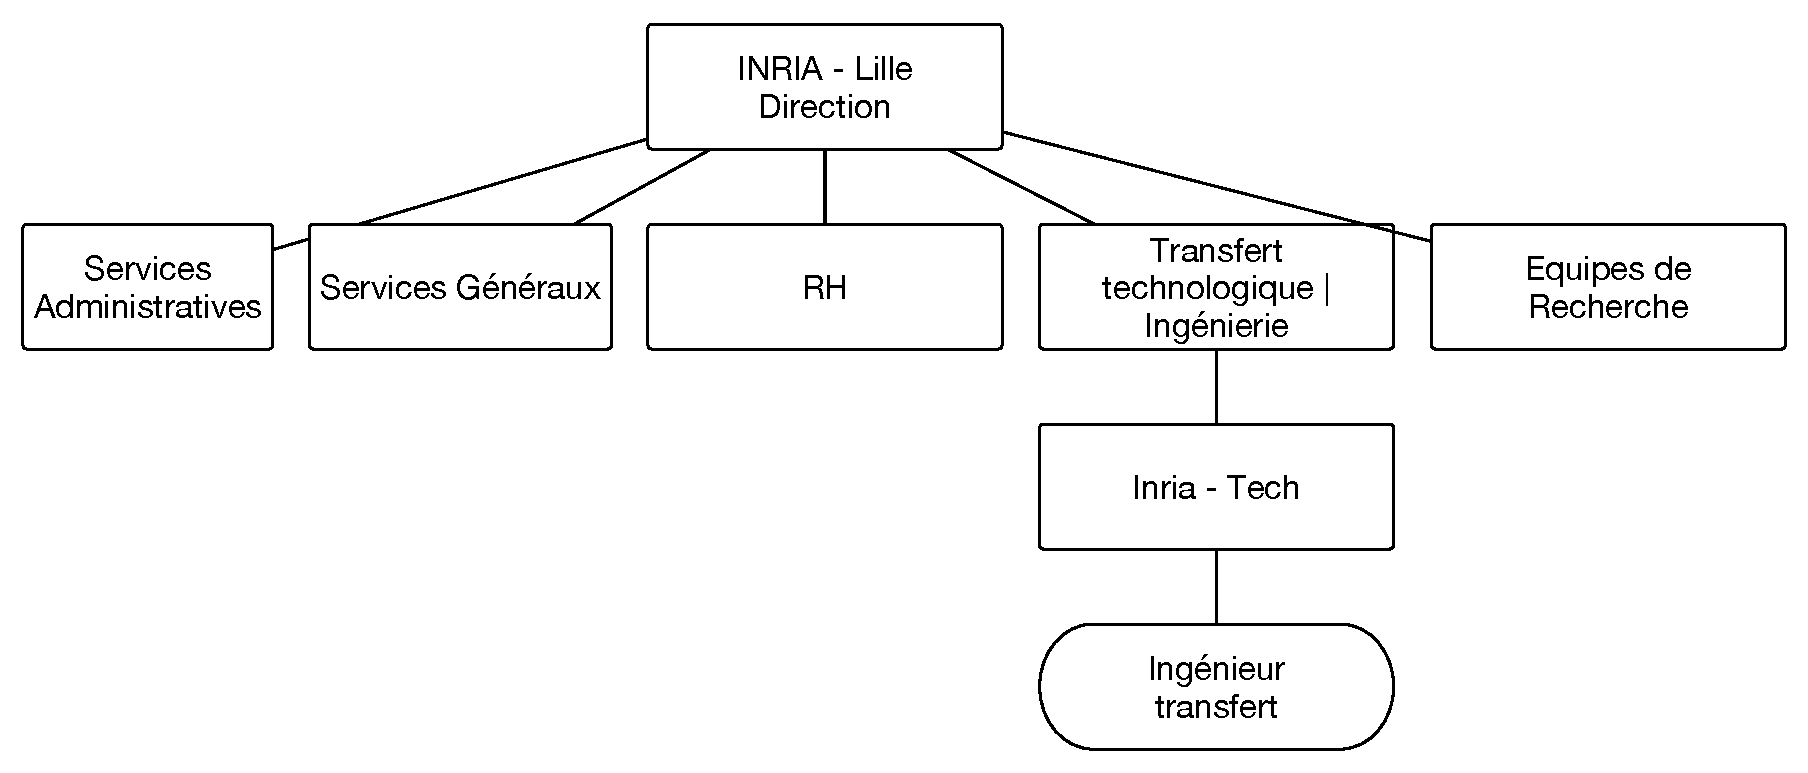
\includegraphics[width=0.60\linewidth]{inria.pdf}
 \caption{Inria - Lille}
 \end{center}
 \end{figure}

	\subsection{Responsabilités}


\begin{table}[!htbp]
\label{my-label}
\begin{tabular}{|lp{12cm}|l|l|l|l}
\cline{1-4}
   & Descriptif des tâches &  \% & Niveau de Responsabilité \footnotemark &  \\ \cline{1-4}
 A& Effectuer de la recherche et du d\'{e}veloppement li\'{e}s \`a des contrats de recherche bilat\'{e}raux avec des entreprises, en particulier des PME  & 60\% &  4&  \\ \cline{1-4}
 B&  Proc\'{e}der \`a la maturation et  à l'adaptation aux besoins des entreprises, de technologies d\'{e}tect\'{e}es dans les \'{e}quipes de recherche  & 30\% & 3 &  \\ \cline{1-4}
 C&  Participer  \`a  des op\'{e}rations de pr\'{e}sentation de l'offre technologique Inria.  &  10\%& 2 &  \\ \cline{1-4}
\end{tabular}
\caption{Responsabilités}
\end{table}


L'ordre d'importance de ces tâches, du point de vue de la gestion de l'Inria, et du point de vue du développement technologique dans la région, devrait être A, C et B. Étant donné que la promotion des solutions existantes est une base nécessaire pour la génération de contrats bilatéraux et pour provoquer l'adoption de nouvelles méthodes de travail. 

\footnotetext{
Niveau de responsabilité
\begin{enumerate} 
	\item de l'application de consignes ou de procédures
	\item de l'amélioration ou de l'optimisation de solutions ou de propositions
	\item de la conception de programmes ou de la définition de cahiers des charges 
	\item de la définition d'orientations ou de stratégies
\end{enumerate}
}

	\subsection{Relations humaines}
	Étant donné qu'Inriatech est une équipe de service d'ingénierie qui travaille de manière transversale, mais qui vise à générer des affinités entre chaque membre et une série d'équipes de recherche, la classification des relations humaines devient compliquée. La ligne entre les relations horizontales, hiérarchiques et externes est très diffuse.
	
		\subsubsection {Relations hiérarchiques}
		\begin{enumerate}
			\item \textbf{De qui recevez-vous vos objectifs, vos instructions ?}
				Les objectifs sont donnés par le résultat des reunions avec des clients et équipes de recherche, en relation aux besoins des clients, possibilités du travail de recherche et alignée avec la vision technologique de chaque équipe et la stratégie de développement associée.
		\item \textbf{Sous quelle (s) forme (s) ?}
				Les objectifs généraux sont décrits dans les contrats bilatéraux entre un partenaire industriel et une équipe de recherche d'Inria. 
				Les objectifs concrets sont décrits et écris dans systèmes de gestion de projets. 
		\item \textbf{Qui évalue votre travail ?}
				Les évaluateurs de mon travaie sont, le responsable du partenaire industriel, le directeur du équipe de recherche lieu au projet, le directeur du Service Transfert pour l'Innovation et Partenariats et le directeur du Service Expérimentation et Développement. 
		\item  \textbf{Eventuellement à qui donnez-vous des objectifs. des instructions, des consignes ?}
			Je n'ai pas des personnes \`a charge.
		\end{enumerate}

	\subsubsection {Relations horizontales } 
	
	\begin{enumerate}
		\item \textbf{ Avec quel (s) service (s) internes êtes-vous en relation pour l'exécution de cette mission ?}
			Les officiers de partenariat  
		\item \textbf{Sous quelle (s) forme (s) ?}
			Sous la forme de reunion formel et cahier des charges. 
	\end {enumerate}
	\begin{enumerate}
		\item \textbf{ Avec quel (s) service (s) internes êtes-vous en relation pour l'exécution de cette mission ?}
			Les membres de chaque équipe de recherche lié avec chaque contrat.
		\item \textbf{Sous quelle (s) forme (s) ?}
			Normalement sous la forme réunion formelle, informelle ou pair programming. 
	\end {enumerate}	

	\subsubsection {Relations extérieures}
		\begin{enumerate}
		\item \textbf{Avec quel (s) partenaire (s) êtes-vous en relation pour l'exécution de cette mission ?}
			Chaque partenaire industriel de chaque contrat de transfert technologique.
		\item \textbf{ Sous quelle (s) forme (s) ?}
			Reunion formelles, informelle, téléphone, courriel et des logiciels de gestion de projet.
		\item \textbf{ Avec quelle fréquence ?}
			Selon le partenaire. Minimalement deux réunions formelles. 
		\end {enumerate}			


	\subsection{Décrivez les principales qualités que vous avez a mobiliser dans cette mission}
			
			\begin{itemize} 				
			\item \textbf{Autonomie et prise de décision} \newline
				Mes projets a INRIA Tech, même comme part d'une équipe, sont assigné individuellement (chaque ingénieur a ses projets), sont aussi sensé a être géré complètement pour l'ingénieur en charge. Chaque un de ces projets que se passent chez les equipes de recherche aussi que chez les clients, demandent une haut autonomie, mobilisation et prise de décision.
				\item \textbf{Apprentissage constant } \newline
				L'environnement de la recherche est fascinant. Chez Inria Lille on a plusieurs équipes de recherche avec des domaines diamétralement différents. Apres avoir travaillé avec quatre équipes différentes avec des domaines si différents comme réseaux d'internet des objets, control adaptatif appliqué aux robots,  interfaces de communication homme-machine non conventionnelles, et implémentations des langages de programmation, j'ai été poussé à apprendre et re-apprendre beaucoup de contenu. 
			\item \textbf{Critique constructive} \newline
				L'ambiance de la recherche, même quand elle est compétitive est aussi très autocritique. Être constructivement critique n'est pas seulement bienvenue, sinon aussi nécessaire.
			\item \textbf{Négociation et prise de décision } \newline
		Etant la personne entre l'équipe de recherche, avec ses ambitions et un partenaire industriel avec des besoins techniques spécifiques, m'a mis dans une situation de négociation  et prise de décision. 
		\end{itemize}

		
	\subsection{Pouvez-vous présenter une situation-problème que vous avez eu a résoudre dans le cadre de cette mission et la façon de dont vous avez procédé?}
	
		Comme exemple de situation a résoudre, j'amène mon première travail à InriaTech. Ce n'est pas le problème le plus compliqué, mais il est très clair et représentatif de mon travail avec les équipes de recherche.  
		
		 Ce premier travail a été un travail de mise a jour de logiciel développé pour des chercheurs mathématiciens / électroniques, pour être applicable sur le domaine de la robotique. 
		J'avais deja été exposé à la robotique pendant mon temps de travaille à l'Ecole des Mines de Douai, mais, par contre je n'ai jamais exposé à ce genre d'algorithmes, a cette partie du développement robotique ou aux genre des équations différentielles utilisées pour la résolution des problématiques. 
		
		Ma mission d'abord a été comprendre la solution proposée par le doctorant, et la faire mature pour pouvoir l'offrir comme possible solution.  
		
		Le code développé pour le thésard  a été impossible à comprendre,  étant un expert mathématicien, mais pas nécessairement expert logiciel, et car sa stratégie  de développement était maintenir les nomenclatures comme dans son article. (Un article mathématique respecte des conventionnes que sont tres bonnes pour le développement mathématique, mais nocives pour le développement logiciel). 
		
		Ma stratégie pour arriver à comprendre le plus vite et faire mon travail en même temps a été l'application des techniques et méthodologies de l'industrie de logiciels, en deux phases : 
		
		\begin{itemize}
				\item Versionner le code, avec un système des versions.
				\item Modifier le code pour le faire fonctionner en mode librairie. 
				\item Développer des test au boîte noire.
				\item Transformer le code en essayent de lui simplifier avec des délégations pertinentes. 
				\item Mise en place de server de integration continue.
		\end {itemize}
		
		Une fois que j'ai amélioré la structure du projet et, parallèlement j'ai lu l'article et appris les notions de base de la méthode, je suis  passé dans une deuxième phase :
		\begin{itemize}
				\item Faire des tests sur les propriétés mathématiques des résultats.
				\item Transformer le code en essayant d'avoir une cohésion sémantique.
				\item Adapter et utiliser dans des expérimentations.
		\end {itemize}
	\subsection {Connaissances mobilisées dans cette mission }
	\begin{itemize} 				
			\item Algorithmique et conception 
					\begin{itemize}
						\item Architecture logicielle robotique 
						\item Développement des algorithmes de Path planning local pour robots differentials 
						\item Implémentation des réseaux  multi-sauts pour objets connectés 
						\item Implémentation des automates finis pour le traitement des signaux
						\item Protocols de consensus pour platforms blockchain 
						\item Conception architecture et développement des langages de consultation 
						\item Administration simples de serveurs de réseaux (windows et linux)
					\end {itemize}
			\item Technologique
					\begin{itemize}
						\item Middleware de développement robotique, ROS 
						\item Système d'exploitation pour IOT, RIOT 
						\item Langage de développement de smart contracts Solidity 
						\item Plateforme de crypto-monnaie Ethereum
						\item Ecriture des grammaires de langages logiciel avec SmaCC (YACC for smalltalk) 
						\item Plusieurs langages de développement Pharo, C, C++, Java, Python, Javascript, Scala
					\end {itemize}
			\item  Recherche 
				\begin{itemize}
						\item Lecture des articles scientifiques 
						\item Ecriture des articles scientifiques (avec deux publications comme auteur principal) 
				\end {itemize}
		\end{itemize}
		


		


\end{document}
